\documentclass[12pt,a4paper,fleqn]{article}
\title{Progress Report}
\author{Syed Ahmad Raza}
\date{2016.11.07}
\usepackage{amsmath}
\usepackage{graphicx}
\begin{document}
	\maketitle
	
	\section*{Numerical integration of sin$(x)$ from 0 to $\pi$\linebreak using two methods}
	The algorithms for numerical integration have been explored and the following two are utilized to calculate the result of integration of sin$(x)$ from $0$ to $\pi$:
	\begin{enumerate}
		\item Trapezoidal rule
		\item Simpson's 1/3 rule
	\end{enumerate}

	Both of these are part of the Newton-Cotes formulas. They involve using an easy approximating function in place of a complicated function or tabulated data.

	The algorithm for both the methods was programmed in C++ and run using GNU C on Cygwin. The interval between the limits was divided into $n$ number of segments with $n$ ranging from $10$ to $1000$.
	
	The results are compared with the analytical solution and graphs are used to display the log of ratio of difference (log$(D)$ between the results versus the log of number of segments (log$(N)$).
	
	\section*{Analytical solution}
	\begin{equation}
	I_A = \qquad\int_{0}^{\pi}\text{sin}(x) = [-\text{cos}(x)]_0^\pi = 2
	\end{equation}
	The analytical solution for this problem is $2$.
	
	\section*{Trapezoidal rule}
	\begin{equation}
	I_N = (b-a)\frac{f(x_0)+2\sum\limits_{i=1}^{n-1}f(x_i)+f(x_n)}{2n}
	\end{equation}
	
	\section*{Simpson's 1/3 rule}
	\begin{equation}
	I_N = (b-a)\frac{f(x_0)+4\sum\limits^{n-1}_{i=1,3,5...}f(x_i)+2\sum\limits_{i=2,4,6...}^{n-2}f(x_i)+f(x_n)}{3n}
	\end{equation}
	
	\section*{Conclusion}
	Simpson's $1/3$ rule is found to converge to the analytical solution faster and is more accurate.
	
	\begin{figure}[!hbp]
		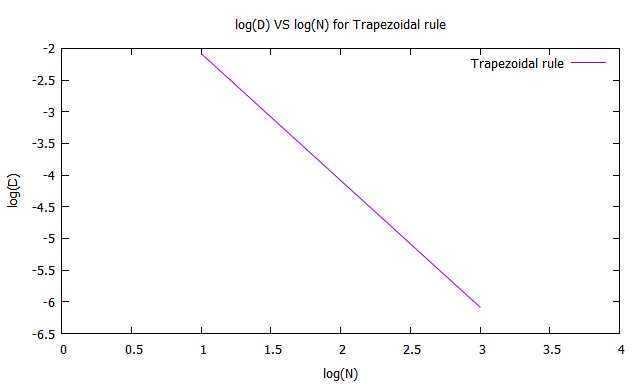
\includegraphics[width=\textwidth]{trapezoidal.png}
		\caption{Plot of log$(D)$ versus log$(N)$ for trapezoidal rule}
	\end{figure}
	
	\begin{figure}[!]
		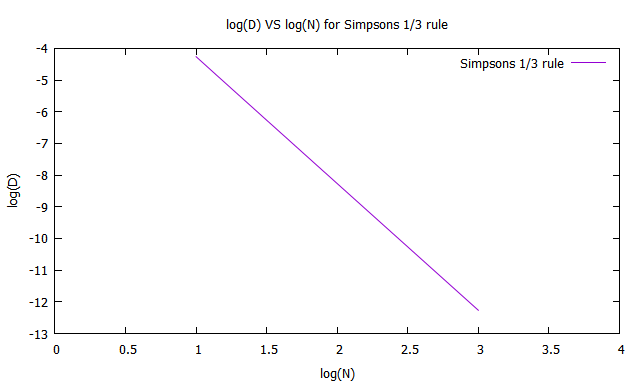
\includegraphics[width=\textwidth]{simpsons13.png}
		\caption{Plot of log$(D)$ versus log$(N)$ for Simpson's 1/3 rule}
	\end{figure}

	\begin{figure}[!]
	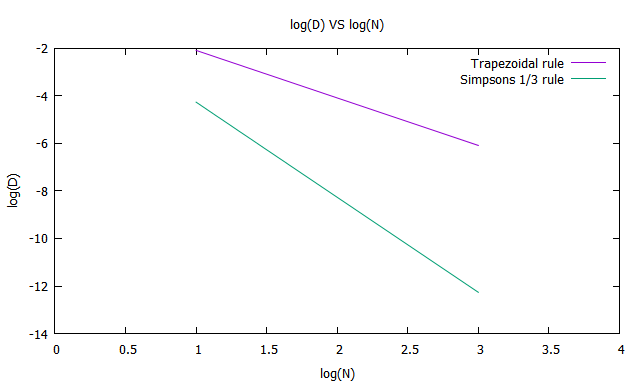
\includegraphics[width=\textwidth]{both.png}
	\caption{Plot of both algorithms together}
	\end{figure}
	
\end{document}